\newpage
\section{Ergebnisse}
Dieses Kapitel stellt die zentralen Ergebnisse des Projekts vor. 
Zunächst wird der entwickelte \acs{aas}-Demonstrator der robocell vorgestellt.
Im Anschluss efolgt die Analyse des eingesetzten \acs{ki}-Modells sowie die Präsentation der beiden Anwendungsfälle. 
Abschließend wird eine Bewertung der verwendeten Softwarelösungen und Tools vorgenommen.

\subsection{AAS-Demonstrator für die robocell}
Im Rahmen dieses Projekts wurde für das Abfüll- und Verschließmodul ein digitaler Zwilling auf Basis der \acs{aas} realisiert.  
Dazu wurde ein \acs{aas}-Demonstrator entwickelt, der sowohl auf standardisierte Templates der \acs{idta} als auch auf individuell angepasste Submodelle zurückgreift.  
Der Zwilling wurde als konkrete Instanz modelliert, um die Anbindung von Echtzeitdaten zu ermöglichen und praxisnahe Anwendungsfälle zu demonstrieren.

Obwohl keine spezifische physische Maschine zugrunde liegt, erlaubt die instanzbasierte Modellierung die Darstellung typischer Maschinendaten wie Prozesswerte, Maschinenstatus oder historische Informationen.  
Eine rein typisierte Modellierung hätte hingegen überwiegend leere Felder zur Folge und wäre für die Veranschaulichung funktionaler Zusammenhänge weniger geeignet.  
Nichtsdestotrotz kann die entwickelte Struktur als Vorlage für zukünftige Projekte dienen.  
Die verwendeten Daten erheben dabei keinen Anspruch auf Vollständigkeit, sondern dienen der exemplarischen Demonstration.

\subsubsection{Systemarchitektur}
Die Gesamtarchitektur des Demonstrators basiert vollständig auf containerisierten Komponenten, wodurch eine skalierbare und modulare Struktur entsteht. 
Als zentrale Plattform zur Verwaltung und Bereitstellung der \acs{aas} dient Eclipse BaSyx. 
Ursprünglich war der AASX Server Blazor vorgesehen, dieser wurde jedoch frühzeitig durch BaSyx ersetzt, da die Plattform eine deutlich flexiblere und umfassendere Umgebung für digitale Zwillinge bietet.

Für die Bereitstellung dynamischer Daten bildeten der Maschinensimulator und der Datengenerator die Grundlage.
Der Maschinensimulator war bereits vorhanden und konnte direkt in das System eingebunden werden. 
Der Datengenerator hingegen wurde im Rahmen des Projekts als Node.js-Anwendung entwickelt. 
Beide Komponenten stellen die Maschinendaten über einen integrierten \acs{opcua} Server bereit und ermöglichen so die Echtzeitkommunikation mit dem digitalen Zwilling. 
Die Datenübertragung erfolgt über die Databridge, welche die Verbindung zwischen den simulierten Datenquellen und den dynamischen Submodellen der \acs{aas} herstellt.

Zur Speicherung und Analyse der Maschinendaten wurde zusätzlich Telegraf eingesetzt, um die Daten in eine InfluxDB zu übertragen. 
Dies ermöglicht nicht nur die Verarbeitung von Echtzeitdaten, sondern auch die Analyse historischer Datenbestände.

Die zugrundeliegende Architektur ist in Abbildung \ref{fig:Systemarchitektur} dargestellt.

\begin{figure}[htbp]
    \centering
        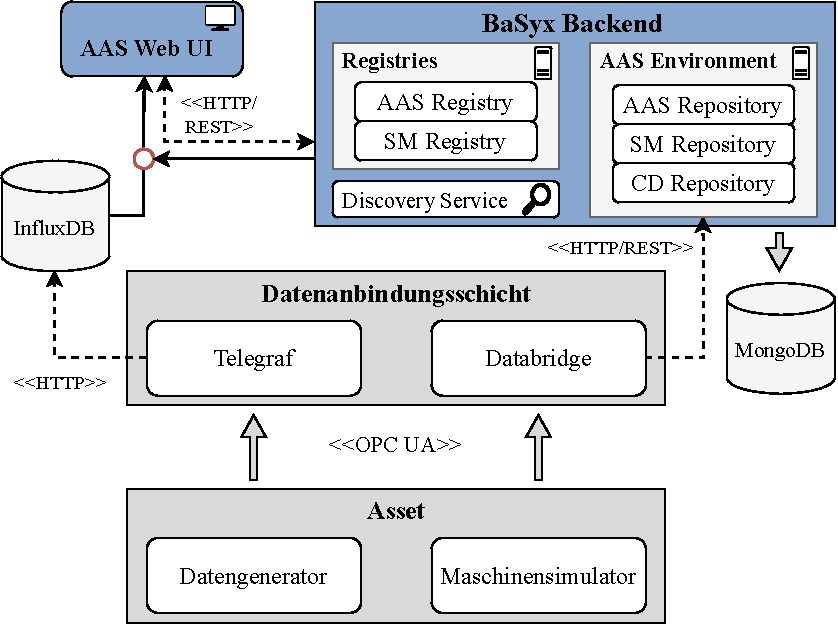
\includegraphics[width=1\textwidth]{Bilder/Ergebnisse/DynamischeDaten/Architektur.pdf}
    \caption{Systemarchitektur AAS-Demonstrator}
    \label{fig:Systemarchitektur}
\end{figure}

Da Einträge in den Discovery Service noch nicht automatisch von stattten gehen wurde zu diesem ein Node.js Skript geschreiben, das diese Funktionalität übernimmt.
Dieses erstellt beim Start der BaSyx-Umgebung automatisch die in einer JSON-Datei hinterlegten Einträge, bei denen das jeweilige Asset mit seiner zugehörogen AAS verknüpft wird.
Dies ist besonders wichtig, um eine AAS finden zu können auch wenn man nur die Asset-ID hat. In dieser Arbeit war dies vor allem zur Abbildung hierarchischer Strukturen sowie für den Anwenungsfall zum DPP notwendig.
Beim Starten der Anwendung werden die Eintröge schließlich automatisch geposted.
In Zukunft erwartet das beu BaSyx das auch automatisch beim Hochladen einer neuen AAS erfolgt und man das nicht mehr selber umsetzen musss, da das sonst sehr aufwendig ist.

Zur Visualisierung der AAS wurde neben der AAS Web UI ebenfalss der Mnestix Browser eingesetzt, da dieser in der Architektur einfach mit dieser ausgetauscht werden kann.
Eine dertailliertere Beschreibung der Tools findet sich in Kapitel !!!.

\subsubsection{AAS-Struktur}

+ Metadaten des Assets und der AAS zB bilder von PE
+ Modellierung untergeordneter komponenten mit eigener AAS
+ Wie QR Code bei groninger. Gibt es nichtr nicht es wurde beispiel id verwendet um das umzusetzten an die MAaschine euiien Code mit der Asset ID
+ Wenn man den scanntn kommt man dahin

\subsubsection{Statische Submodelle}

Die statische Modellierung wurde vollständig mit dem Package Explorer durchgeführt. 
Alle relevanten statischen Informationen wurden manuell eingetragen. 
Als Hauptdatenquellen dienten technische Dokumentationen der robocell, insbesondere die Betriebsanleitung, sowie Informationen aus dem \acs{plm}-System Agile.

\subsubsection*{Typenschild}
\vspace{-0.5em}

\subsubsection*{\acs{bom}}
\vspace{-0.5em}

\subsubsection*{Technische Daten}
\vspace{-0.5em}

\subsubsection*{Dokumentation}
\vspace{-0.5em}

\subsubsection*{3D-Modelle}
\vspace{-0.5em}

\subsubsection*{Wartung}
\vspace{-0.5em}

\subsubsection{Dynamische Submodelle}
Eine rein statisch modellierte \acs{aas} bildet lediglich die Struktur und Metadaten eines Assets ab und erfüllt damit noch nicht die Anforderungen an einen digitalen Zwilling gemäß der in Kapitel \ref{sec: DT} dargestellten Klassifizierung. 
Erst durch die Integration von Echtzeitdaten sowie der Möglichkeit zur Interaktion mit dem physischen System entsteht eine digitale Repräsentation, die über eine reine Beschreibung hinausgeht.

Die Erweiterung der \acs{aas} um dynamische Daten wurde in dieser Arbeit durch die Umsetzung von drei Submodellen realisiert, die nachfolgend vorgestellt werden. 
Diese wurden zunächst im Package Explorer strukturiert und anschließend zur Laufzeit in der BaSyx-Umgebung mit simulierten Daten befüllt bzw. aktualisiert.

\subsubsection*{Prozessdaten}
\vspace{-0.5em}

Die Maschine wurde durch einen Datengenerator sowie einen Maschinensimulator repräsentiert. 
Im Submodell Prozessdaten werden simulierte Werte wie Füllstand, Durchfluss, Anzahl abgefüllter Einheiten sowie Druck erfasst. 
Diese Werte werden mithilfe der Databridge aktualisiert, die ein Subscription-Modell verwendet. 
Änderungen werden sofort erkannt, transformiert und in die entsprechenden Properties des Submodells geschrieben, genauer gesagt in das Submodel Repository der AAS Environment.

Der Datengenerator erzeugt Daten im Sekundentakt. 
In der AAS Web UI wurde ein Plugin implementiert, das diese Werte visualisiert. 
Die Anwendung fragt die \acs{aas}-Daten der hinterlegten Services in einem konfigurierbaren Intervall (z. B. alle 4 Sekunden) ab und aktualisiert die Anzeige entsprechend.

\begin{figure}[htbp]
    \centering
        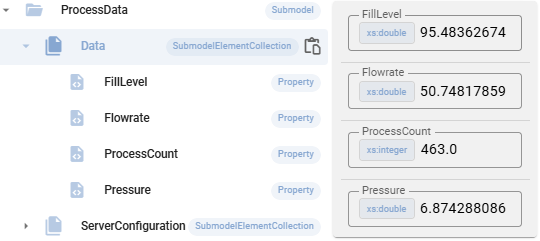
\includegraphics{Bilder/Ergebnisse/DynamischeDaten/ProcessData/Visualisierung.PNG}
    \caption{Systemarchitektur AAS-Demonstrator}
    \label{fig:Systemarchitektur}
\end{figure}

\subsubsection*{Kontrollkomponente}
\vspace{-0.5em}
Ein vergleichbarer Mechanismus wie bei den Prozessdaten kommt auch im Submodell Kontrollkomponente zum Einsatz. 
Die Zustandsdaten des Maschinensimulators werden über \acs{opcua} abgefragt und mithilfe der Databridge in das entsprechende Submodell der \acs{aas} geschrieben. 
Da der Simulator numerische Zustände liefert, erfolgt eine semantische Umwandlung mittels JSONata, um diese in sprechende Zustandsbezeichnungen wie Execute, Stopped oder Suspending zu überführen.

Die Zustände orientieren sich am PackML-Standard, der insgesamt 17 definierte Maschinenzustände umfasst. 
Diese standardisierte Struktur ermöglicht eine konsistente Erfassung und Interpretation des Maschinenstatus und wird auch für die robocell-Linie eingesetzt.
Der Maschinenstatus selbst ist in einer \acs{smc} organisiert, in der eine Property den aktuellen Zustand abbildet.

Zur Visualisierung wurde ein bestehendes Vue.js-Plugin verwendet, das ursprünglich im Rahmen eines Forschungsprojekts an der Hochschule für Technik und Wirtschaft Berlin entwickelt wurde \cite{HTW1}\cite{HTW2}. 
Da das Plugin nicht weiter gepflegt wurde, wurde es funktional angepasst und in die AAS Web UI integriert, um es für den Demonstrator nutzbar zu machen.

Die aktuellen Zustandsinformationen werden darin visuell in Form eines PackML-Zu\-standsautomaten dargestellt, wie Abbildung \ref{fig:PackMLZustandsautomat} zeigt. 
Um Änderungen direkt anzuzeigen, wurde eine Polling-Logik implementiert, die den Maschinenstatus in regelmäßigen Abständen vom Submodel Repository der AAS Environment abfragt.

\begin{figure}[htbp] 
    \centering 
        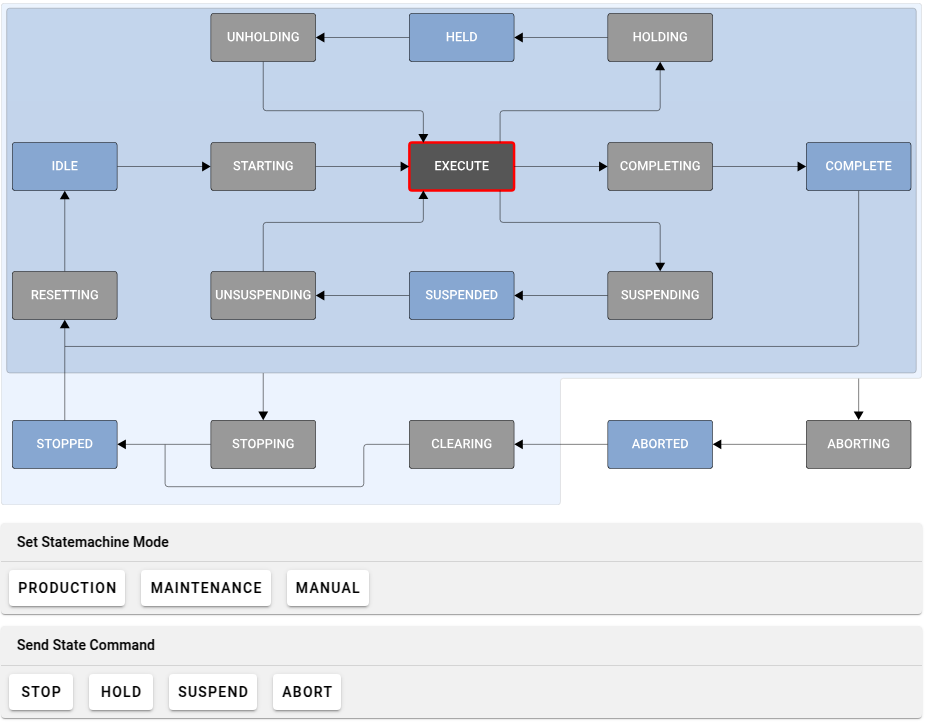
\includegraphics[width=1\textwidth]{Bilder/Ergebnisse/DynamischeDaten/Kontrollkomponente/PackMl.PNG} 
    \caption{Plugin Submodell Kontrollkomponente} 
    \label{fig:PackMLZustandsautomat} 
\end{figure}

Wie auch in der Abbildung zu erkennen besteht neben der Visualisierung auch die Möglichkeit, den Maschinenmodus direkt über die AAS Web UI zu ändern. 
Über interaktive Schaltflächen können Nutzer konforme Zustandsübergänge gemäß PackML auslösen. 
Befindet sich die Maschine beispielsweise im Zustand Execute, sind die Befehle Stop, Hold, Suspend und Abort möglich. 
Nicht erlaubt wären direkte Übergänge zu Zuständen wie Idle, Reset oder Completed.

Zusätzlich kann der Maschinenmodus gesetzt werden. 
Die vorliegende Umsetzung unterstützt drei Betriebsmodi: Produktion, Manuell und Wartung. 
Diese werden analog zum Maschinenstatus über eine entsprechende Property im Submodell Kontrollkomponente im Submodel Repository der AAS Environment verwaltet.

Im Demonstrator wird der Maschinenzustand direkt über eine WebSocket-Verbindung vom Plugin an den Maschinensimulator übermittelt und ohne weitere Prüfung übernommen. 
Dadurch entsteht eine einfache Feedback-Schleife zwischen Benutzeroberfläche und Simulator, die eine direkte Steuerung aus der \acs{aas} ermöglicht.

In einer realen Maschinenumgebung würde der Steuerbefehl zunächst mit einem geeigneten Industrieprotokoll wie \acs{opcua} an die speicherprogrammierbare Steuerung (SPS) der Maschine übertragen werden müssen. 
Nach erfolgreicher Validierung und der Durchführung notwendiger Operationen, etwa dem Abschalten von Motoren oder dem Schließen von Ventilen, würde der neue Zustand gesetzt und anschließend an die \acs{aas} zurückgemeldet werden.

\subsubsection*{Zeitreihendaten}
\vspace{-0.5em}
Das dritte Submodell, das ebenfalls als dynamisches Submodell eingeordnet werden kann, ist die Darstellung von Zeitreihendaten. 
Datengrundlage bilden erneut die simulierten Prozesswerte des Datengenerators.
Diese werden kontinuierlich über Telegraf in eine InfluxDB geschrieben und stehen somit für zeitbasierte Auswertungen zur Verfügung.

Die AAS Web UI ermöglicht den direkten Zugriff auf diese Daten. 
Über die im Submodell hinterlegten Parameter kann eine gezielte Abfrage an die Datenbank gestellt werden. 
Die Ergebnisse werden anschließend im Visualisierungsbereich der Benutzeroberfläche dargestellt. 
Dabei muss das gewünschte Segment sowie die darzustellenden Messgrößen ausgewählt werden.

Zur Visualisierung stehen verschiedene Diagrammtypen zur Verfügung. 
Die Datenbankabfrage selbst ist im LinkedSegment hinterlegt und definiert den Zeitraum, über den die Daten abgefragt werden.
Unabhängig davon kann der Zeitraum, der in der Visualisierung angezeigt wird, individuell angepasst werden.

Abbildung \ref{fig:LiniendiagrammBaSyx} zeigt die Darstellung von Druck und Temperatur über einen Zeitraum von einer Minute in einem Liniendiagramm.

\begin{figure}[htbp]
    \centering
        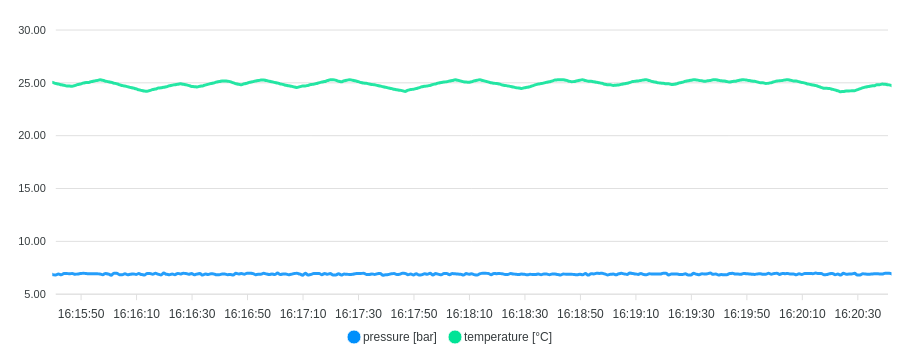
\includegraphics[width=1\textwidth]{Bilder/Ergebnisse/DynamischeDaten/ZeitreihenDaten/line.png}
    \caption{Zeitreihendaten in der AAS Web UI}
    \label{fig:LiniendiagrammBaSyx}
\end{figure}

Ein wesentlicher Vorteil dieser Umsetzung ist die Entkopplung der Datenspeicherung von der AAS selbst. 
Da die \acs{aas} keine Datenbank ist, eignet sich dieser Mechanismus besonders für die Integration großer oder historischer Datenmengen. 
Er lässt sich flexibel auf beliebige Datensätze anwenden und erweitert so die Funktionalität der \acs{aas} sinnvoll um zeitbasierte Analyse- und Visualisierungsoptionen.

%KI-Modell
\subsection{Evaluation des KI-Modells}
\subsubsection{Bewertung des prototypischen KI-Einsatzes}
\subsubsection{Ausblick: Predictive Maintenance}
\subsubsection{Weiterführende Einsatzmöglichkeiten}

% Digitaler Produktpass
\newpage
\subsection{Anwendungsfall Digitaler Produktpass}
\subsubsection{Abbildung des PCF}
Zur Abbildung des \acs{pcf} der Gesamtmaschine wurde ein Mechanismus in der AAS Web UI integriert. 
Im Visualisierungsbereich wurde eine Schaltfläche implementiert, über die die Aggregation der CO\textsubscript{2}-Äquivalente ausgelöst werden kann. 
Beim Betätigen dieser wird eine \acs{http}-GET-Anfrage an den Microservice gesendet, der die Berechnung durchführt.

Der Microservice, der ebenfalls als Docker-Container implementiert wurde, reagiert auf die Anfrage und startet den Berechnungsprozess. 
Der Ablauf ist in Abbildung \ref{fig:SequenzdiagrammPCF} als Sequenzdiagramm dargestellt.

\begin{figure}[htbp]
    \centering
        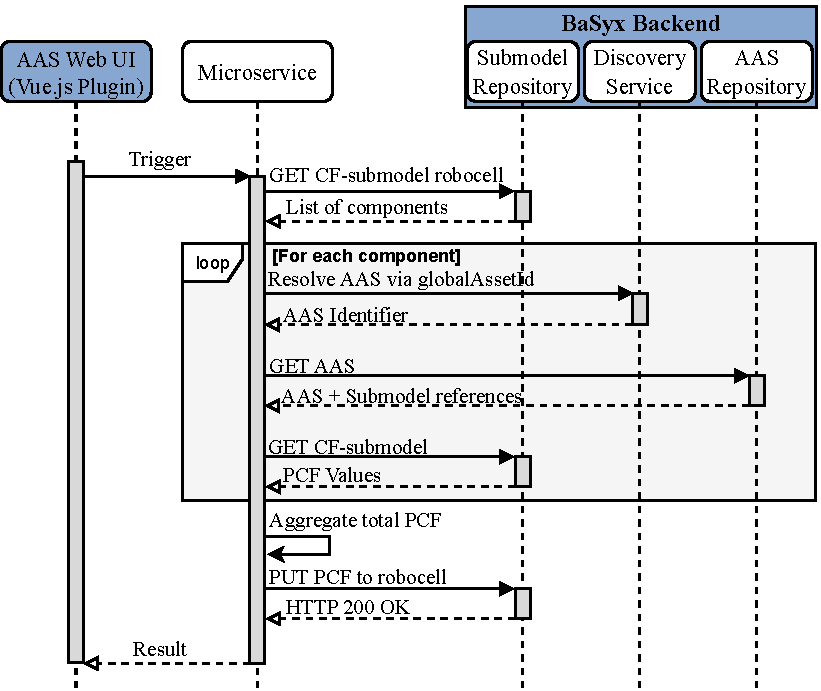
\includegraphics[width=1\textwidth]{Bilder/Ergebnisse/DPP/AggregationNue.pdf}
    \caption{Sequenzdiagramm zur Aggregation des PCF}
    \label{fig:SequenzdiagrammPCF}
\end{figure}

Der Microservice nutzt die \acs{rest}-Schnittstelle des Submodel Repositories der AAS Environment, um zunächst alle in der Komponentenliste des \acs{cf}-Submodells der robocell hinterlegten Komponenten auszulesen. 
Mithilfe des Discovery Service werden auf Basis ihrer globalAssetIds die zugehörigen Komponenten-\acs{aas} identifiziert und anschließend vom AAS Repository abgerufen.
Für jede dieser Komponenten wird geprüft, ob ein \acs{cf}-Submodell vorhanden ist. 
Falls dies zutrifft, wird das Submodell ausgelesen und die enthaltenen \acs{pcf}-Werte extrahiert.

Aus den ermittelten Einzelwerten berechnet der Microservice die aggregierten CO\textsubscript{2}-Äquivalente für die Phasen Produktion, Material sowie Cradle to Gate. 
Die berechneten Werte werden abschließend in das \acs{cf}-Submodell der Haupt-\acs{aas} der robocell geschrieben und stehen dort strukturiert zur Verfügung.

Nach Abschluss der Berechnung sendet der Microservice eine Bestätigung an das Plugin zurück. 
Dieses reagiert darauf, indem es das aktualisierte \acs{cf}-Submodell über die \acs{rest}-Schnittstelle der AAS Environment erneut abfragt. 
Die relevanten Submodellelemente werden dabei herausgefiltert und in der Benutzeroberfläche aktualisiert. 
Dadurch werden die aggregierten \acs{pcf}-Werte unmittelbar sichtbar, ohne dass ein manuelles Neuladen erforderlich ist.

Abbildung \ref{fig:PluginAggregation} zeigt die entsprechende Visualisierung. 
Auf der linken Seite sind die berechneten CO\textsubscript{2}-Äquivalente dargestellt, auf der rechten Seite die zugehörigen Lebenszyklusphasen.

\begin{figure}[htbp]
    \centering
        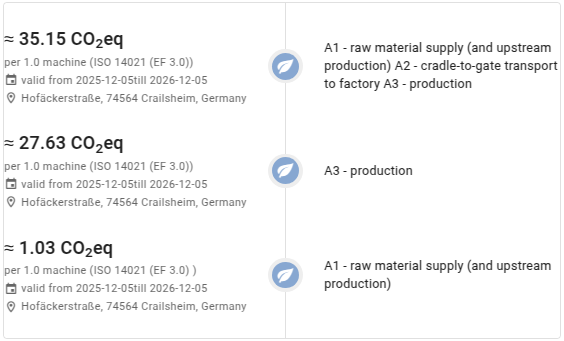
\includegraphics{Bilder/Ergebnisse/DPP/PluginAggregation.png}
    \caption{Visualisierung der aggregierten PCF-Werte im Plugin}
    \label{fig:PluginAggregation}
\end{figure}

Die beschriebene Lösung ermöglicht es, den \acs{pcf} dynamisch auf Basis der in der Komponentenliste referenzierten Steuerungselemente zu berechnen. 
Auch wenn derzeit nur acht Siemens-Komponenten berücksichtigt werden, lässt sich die Liste bei Verfügbarkeit weiterer Komponenten-\acs{aas} unkompliziert erweitern, sodass sukzessive die gesamte Maschine in die Berechnung einbezogen werden kann.

Perspektivisch lässt sich die Berechnung zudem um weitere Lebenszyklusphasen wie Nutzung oder Entsorgung ergänzen, um eine ganzheitliche Betrachtung von der Herstellung bis zum Lebensende eines Produkts bzw. einer Maschine zu ermöglichen.
Darüber hinaus könnte auch der \acs{tcf} berücksichtigt werden, beispielsweise im Rahmen der Auslieferung einer Maschine, wodurch eine noch umfassendere Bilanzierung der Umweltauswirkungen ermöglicht wird.

\subsubsection{Rollenbasierter Zugriff auf Submodelle}
Eine Möglichkeit, die im \acs{dpp} enthaltenen Informationen einzusehen, bietet die AAS Web UI. 
Ist \acs{rbac} aktiviert, wird der Benutzer beim Aufruf der Oberfläche zur Keycloak-Anmeldeseite weitergeleitet. 
Wie in Abbildung \ref{fig:KeycloakAnmeldeSeite} dargestellt, kann sich der Nutzer dort mit dem in Keycloak hinterlegten Benutzernamen und Passwort authentifizieren.

\begin{figure}[htbp]
    \centering
        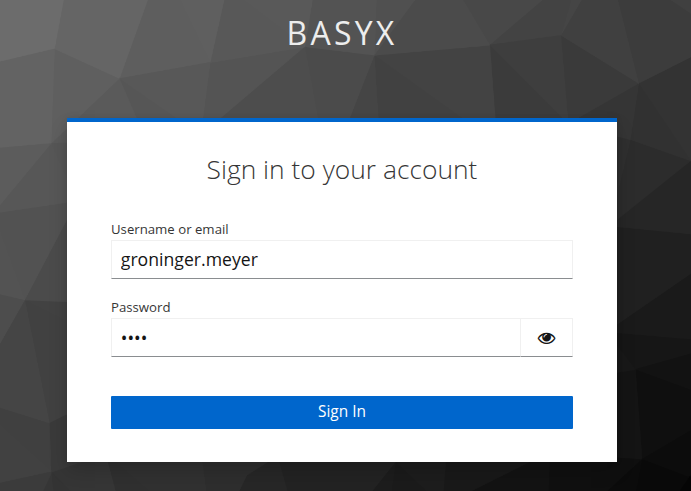
\includegraphics[width=0.7\textwidth]{Bilder/Ergebnisse/DPP/KeycloakAnmeldeSeite.png}
    \caption{Keycloak-Anmeldeseite für die AAS Web UI}
    \label{fig:KeycloakAnmeldeSeite}
\end{figure}

Nach erfolgreicher Anmeldung erhält der registrierte Client (AAS Web UI) ein Zugriffstoken, das die Rolleninformationen des Nutzers enthält.  
Dieses Token wird im Hintergrund an die angebundenen BaSyx-Komponenten (z.\,B. AAS Environment, Registries) weitergegeben.  
Die Entscheidung über die tatsächliche Zugriffsberechtigung trifft dabei nicht die AAS Web UI, sondern der jeweilige Service, indem er die im Token enthaltenen Rollen gegen die hinterlegten RBAC-Regeln prüft.
Ist keine Konfiguration hinterlegt, werden keine AAS angezeigt.

Meldet sich beispielsweise der Benutzer customer.doe an, so sieht er zwar den \acs{dpp}, jedoch nur die Submodelle, die in den RBAC-Konfigurationsdateien für die Rolle Kunde freigegeben sind. 
Dazu zählen beispielsweise das Typenschild, Technische Daten oder der \acs{cf}. 
Andere Submodelle wie 3D-Modelle oder Wartungsinformationen werden nicht angezeigt und erscheinen als nicht gefunden. 
Darüber hinaus besitzt der Benutzer lediglich Leserechte, sodass keine Änderungen an den Inhalten vorgenommen werden können. 
Versucht er, eine neue \acs{aas} über die Benutzeroberfläche hochzuladen, wird der Vorgang mit einem \acs{http}-Fehler 403 abgelehnt.

Neben dem Zugriff über die AAS Web UI ist auch ein direkter Zugriff auf die BaSyx-Komponenten über die \acs{api} möglich.
Dies ist insbesondere für technische Clients oder externe Anwendungen relevant, die automatisiert auf die im \acs{dpp} enthaltenen Informationen zugreifen sollen.
In diesem Fall muss ein Zugriffstoken aktiv über den Token-Endpunkt des entsprechenden Realms in Keycloak angefordert und anschließend im \acs{http}-Header der Anfrage übermittelt werden.

Für diesen Anwendungsfall wurden in Keycloak drei Clients eingerichtet, denen jeweils ein Service Account zugewiesen wurde.
Diese Service Accounts sind mit den Rollen Groninger-Mitarbeiter, Service-Techniker und Kunde ausgestattet.
Durch die Zuweisung der Rollen erhalten die Clients somit dieselben Zugriffsrechte wie die entsprechenden Benutzerkonten.

Zum Testen von Client-Zugriffen wurde das Tool Postman verwendet.
Dabei muss zunächst ein Zugriffstoken über den Token-Endpunkt des entsprechenden Realms in Keycloak angefordert werden, abhängig davon, welcher Client den \acs{api}-Aufruf durchführen soll.
Die Authentifizierung erfolgt über das OAuth 2.0 Password Grant-Verfahren, das die Grundlage des in Keycloak verwendeten OpenID Connect-Protokolls bildet.

Für die Anfrage eines Tokens in Postman sind folgende Informationen erforderlich:

\begin{itemize}[noitemsep, leftmargin=*]
    \item \textbf{Client-ID und Client-Secret:} Diese dienen zur Authentifizierung des Clients. Die Client-ID entspricht dem Namen des Clients in Keycloak, während das zugehörige Secret automatisch generiert wird und dort eingesehen werden kann.
    \item \textbf{Benutzerkonto:} Ein Benutzername und Passwort eines Kontos, das der im Service Account zugewiesenen Rolle entspricht.
\end{itemize}

Im Folgenden werden die Zugriffsrechte am Beispiel des Service Techmnikers gezeigt.
Nach dem Erhalt eines Tiokens kkann eine Anfrage gestellt werden.

Get auf Wartungs Submodell mit erfolgreicher Anfrage 

Put mit neuem Wartungtsdatum

Get auf CF Submodell mit Fehler

Delete Versuch mit Fehler


Zeigt dass sich differenzierte Zugriffskontrollen auf Submodell-Ebene technisch realisieren lassen. 
Dies bietet Potenzial für zukünftige Szenarien, bei denen sensible Nachhaltigkeitsdaten nur bestimmten Akteuren entlang der Wertschöpfungskette zugänglich gemacht werden sollen.

\subsection{Anwendungsfall automatisierte Generierung der AAS}
% \subsection{Einsatzmöglichkeiten von KI im Kontext der Verwaltungsschale}
% \subsubsection{Generierung von Verwaltungsschalen}
% \subsubsection{Anomaliererkennung}
% \subsubsection{Weiterführende Einsatzmöglichkeiten}

%Evaluation der eingesetzten Software
\subsection{Evaluierung eingesetzter Tools und Software}
\subsubsection{AASX Package Explorer}
\subsubsection{Eclipse AASX Server}
\subsubsection{BaSyx}
\subsubsection{Mnestix Browser}
Optional davor halt nicht drauf eingeganen\dots